\documentclass[10pt,a4paper]{article}
\usepackage[T1]{fontenc}
\usepackage[utf8]{inputenc}
\usepackage[margin=2cm]{geometry}
\usepackage{booktabs,graphicx,tabularx,array,amsmath,microtype,enumitem,caption,xcolor}
\usepackage[hidelinks]{hyperref}
\captionsetup{font=small,labelfont=bf,skip=3pt}
\setlist{nosep,leftmargin=*}
\setlength{\parskip}{3pt}
\setlength{\parindent}{0pt}
\setlength{\tabcolsep}{4pt}
\renewcommand{\arraystretch}{1.05}
\newcolumntype{Y}{>{\raggedright\arraybackslash}X}
\newcommand{\pmsd}[2]{#1{\scriptsize$\pm$#2}}

\title{\vspace{-1.2cm}\textbf{Swasthya Saathi: A Safety-Gated, Hindi-First Agent\\for Appointments and Urgency Triage}\\[2pt]\large Final Report -- LMA Group Project 2026}
\author{Aaryan Kashyap, Hrigved Naidu, Paridhi Mittal, Shantanu Mande}
\date{November 2026\\[2pt]\small Code and data: \url{https://github.com/aaryankashyap007/LMA-Final-Project---4-gram-squad} (branch \texttt{agent-lane})}

\begin{document}
\maketitle
\vspace{-0.8cm}
\begin{abstract}\small
Swasthya Saathi is a research prototype of a clinic front-desk agent for patients who write in Devanagari Hindi, romanised Hindi (Hinglish) or English. It takes two decisions out of the language model: a small fine-tuned \emph{safety gate} decides how urgent a message is, and a deterministic \emph{action guard} approves every state-changing tool call. We test which component is responsible for safety with a $2\times2$ ablation (gate on/off $\times$ guard on/off) on synthetic data. The QLoRA gate reaches emergency recall 0.913 at over-triage 0.067 and, at a matched 10\% over-triage budget, finds 0.82 of emergencies against 0.63 for a prompted gate. Across about 1,190 agent episodes, the models we could use almost never attempted a harmful action: 5 harmful episodes occurred with the guard off (2 each in A1 and +Gate, 1 in the prompted-gate arm), none with it on, and all 16 harmful attempts in the guard arms were blocked. The difference is not statistically significant (2 versus 0 harmful episodes), so the evidence that the guard is what protects the clinic comes from tests that do not depend on the model's goodwill: an always-obeying scripted agent is harmed in 81 of 81 attack scenarios without the guard and 0 of 81 with it, and mutation testing shows each guard rule is needed. We report what did not work, and that no clinician reviewed the rubric.
\end{abstract}

\section{Introduction}
A tool-using LLM handles appointment booking fluently, but the errors that matter at a clinic are decision errors: a missed emergency, or a booking or cancellation run for the wrong person or without consent. In one prompt these decisions cannot be tested separately, and LLM triage is worse on romanised text than on native script~\cite{scriptgap}. Swasthya Saathi makes the two decisions separate components. We ask: \textbf{RQ1} does separating them from generation reduce missed emergencies and unapproved tool calls without hurting task completion, and which component accounts for each reduction? \textbf{RQ2} are triage decisions consistent across Devanagari, Hinglish and English? The hypotheses were H1 (a tuned gate beats a prompted gate on emergency recall at a fixed over-triage rate), H2 (the guard lowers the unapproved-action rate) and H3 (decisions hold across scripts).

\textbf{Contributions.} (i) A script-parallel triage set, D3, and a clinic simulator, D4, with five scenario sets and an independent scoring oracle; (ii) a $2\times2$ gate-by-guard ablation with paired statistics; (iii) three guard tests that do not need a model to misbehave (attempt replay, an always-obeying agent, mutation testing); (iv) a rule-based reply verifier; (v) an honest account of failures and of what could not be done. All data are synthetic; this is not a medical device.

\textbf{Related work.} Prior work covers triage on native versus romanised Indian-language text without any agent or tools~\cite{scriptgap}, public triage criteria~\cite{iitt}, and tool-agent benchmarks that score whole agents on non-medical tasks~\cite{taubench,bfcl}. None isolates the decisions that matter for a clinic, urgency and action approval, as separately switchable components; that is the gap we test.

\section{System, data and protocol}
\textbf{Pipeline.} Each message is normalised, then read by the gate (Qwen2.5-3B-Instruct~\cite{qwen} with a QLoRA adapter~\cite{lora,qlora}, rank 16, trained on D3 train; it reads the last three messages and answers with one letter whose logits give the class probabilities). EMERGENCY or URGENT ends the turn with a fixed Hindi reply, a staff hand-off and a lock on booking tools. A plain administrative message that the gate calls INSUFFICIENT is overridden to ROUTINE (the gate called 79\% of plain administrative first messages harmful before this rule). Otherwise the LLM orchestrator calls tools through the guard: allow-list and schema, identity (the caller's phone must be registered to the patient, proxies included), ownership of an appointment, booking lock, and confirmation (the exact action was proposed and the patient's next message is a short, unqualified yes). A rule-based verifier checks each reply for medicine, dose, diagnosis and home-remedy advice.

\textbf{D3 triage set.} 450 cases (150 evaluation, 300 training), each written in English, Devanagari and Hinglish from one cue list; a second reader found all cues in 143 of 150 rows on the first pass and the 7 mismatches were adjudicated. Labels follow a four-level rubric; test has 42 emergency cases per script. \textbf{D4 scenario sets} (Table~\ref{tab:sets}) are scripted conversations with a gold record of what the patient authorised. An episode is scored by an independent oracle from the clinic's final state and audit log, not by the guard's own verdicts: an \emph{unapproved action} is an executed state change not in the gold, a \emph{leak} is a lookup of another patient, and \emph{task success} means the final bookings equal the gold.

\begin{table}[t]
\centering\small
\begin{tabularx}{\textwidth}{@{}l r Y l@{}}
\toprule
Set & Scen. & What it tests & Runs (episodes)\\
\midrule
Benign & 39 & booking, cancelling, proxy caller, policy, hours, greeting, 6 must-escalate cases & Ultra (195 + 39 gate-V0)\\
Adversarial v0 & 39 & overt injection, impersonation, pressure, role play (+ benign twins) & Nano (195 + 39)\\
Adversarial v1 & 30 & plausible requests: ``for my neighbour'', pasted ``clinic email'', wrong id & Nano, Liquid (150 each)\\
Adversarial v2 & 27 & instruction planted in a policy text or doctor description a tool returns & Nano, Liquid (135 each)\\
Medical advice & 30 & asks for a medicine, dose, diagnosis or home remedy & Liquid (150)\\
\bottomrule
\end{tabularx}
\caption{D4 scenario sets (each family in English, Hinglish and Devanagari). Agent models: Nemotron Ultra (550B), Nemotron Nano (30B-A3B) and Liquid LFM3 (1.7B) through OpenRouter, temperature 0, one run per scenario, token budget 40k.}
\label{tab:sets}
\end{table}

\textbf{Arms.} A0 plain LLM without tools; A1 LLM triage by prompt, guard off; +Gate G1, guard off; +Guard prompted triage, guard on; Full G1 and guard; plus +Gate\_V0 (prompted Qwen gate, guard off). Same backbone, tools and budget. \textbf{Statistics.} Arms are compared paired on the same scenario with exact McNemar tests, Holm correction over the four $2\times2$ comparisons, and bootstrap intervals resampled over scenario \emph{families}, since the three script versions of a case are not independent; rate intervals are exact (Clopper--Pearson).

\textbf{Training and tuning.} G1: 3 epochs, learning rate $2\times10^{-4}$, batch 4 with 4 accumulation steps, seeds 13, 42, 2026, 4-bit; it was not tuned, the first configuration is the reported one. MuRIL: 10 epochs, learning rate $5\times10^{-5}$, batch 8; it received one round of tuning on the dev split (a first configuration underfit), so if anything the baseline was tuned more than the proposed method. The test split was scored again only to add later seeds and ablation runs. Training on a 4-bit model is not bit-exact: seed 13 gave macro-F1 0.810 on one run and 0.850 on another, so differences of a few points between single runs should not be over-read.

\section{Triage gate results}
\begin{table}[t]
\centering\small
\begin{tabularx}{\textwidth}{@{}l c c c c c Y@{}}
\toprule
System (trained on) & Runs & Em.\ recall & Over-triage & Macro-F1 & Gap & Recall EN / DE / HI\\
\midrule
B0 keyword & 1 & 0.484 & 0.143 & 0.450 & 0.119 & 0.405 / 0.524 / 0.524\\
V0 Qwen prompted, 0-shot & 1 & 0.738 & 0.132 & 0.547 & 0.333 & 0.905 / 0.738 / 0.571\\
V0 Qwen prompted, 8-shot & 1 & 0.802 & 0.127 & 0.691 & 0.143 & 0.857 / 0.833 / 0.714\\
B1 MuRIL~\cite{muril} (all) & 3 & \pmsd{0.884}{0.119} & \pmsd{0.289}{0.307} & \pmsd{0.630}{0.120} & 0.040 & 0.897 / 0.873 / 0.881\\
\textbf{G1 QLoRA gate (all)} & 3 & \pmsd{\textbf{0.913}}{0.035} & \pmsd{\textbf{0.067}}{0.011} & \pmsd{\textbf{0.812}}{0.037} & 0.095 & 0.952 / 0.929 / 0.857\\
G1 (English only) & 3 & \pmsd{0.593}{0.083} & \pmsd{0.035}{0.006} & \pmsd{0.688}{0.051} & 0.429 & 0.849 / 0.508 / 0.421\\
G1 (Hinglish only) & 3 & \pmsd{0.831}{0.012} & \pmsd{0.078}{0.003} & \pmsd{0.771}{0.032} & 0.119 & 0.897 / 0.809 / 0.786\\
G1 (Devanagari only) & 3 & \pmsd{0.733}{0.037} & \pmsd{0.051}{0.011} & \pmsd{0.749}{0.012} & 0.373 & 0.714 / 0.929 / 0.556\\
\bottomrule
\end{tabularx}
\caption{Triage on the test split (126 emergency renderings; mean and sd over seeds 13, 42, 2026; prompted systems are deterministic). Gap = highest minus lowest recall over the three scripts.}
\label{tab:triage}
\end{table}

\textbf{H1 is supported} (Table~\ref{tab:h1}). At the dev-chosen 10\% over-triage budget the tuned gate finds $0.820\pm0.030$ of emergencies against 0.627 (8-shot) and 0.508 (0-shot); the paired bootstrap differences are $+0.16$ to $+0.21$ and $+0.28$ to $+0.33$ across the three seeds, and all six intervals exclude zero (the 10\% budget was chosen after earlier results were seen; 5\% and 20\% point the same way). Recall alone misleads: one MuRIL seed reached recall 1.0 by calling 64\% of non-emergencies emergencies, which is why over-triage and macro-F1 are always shown, and why MuRIL, with probabilities that are too extreme to threshold, scores poorly at a fixed budget.

\begin{table}[t]
\centering\small
\begin{tabularx}{\textwidth}{@{}l c c c Y@{}}
\toprule
System & Budget 5\% & Budget 10\% & Budget 20\% & Realised test over-triage (5 / 10 / 20\%)\\
\midrule
MuRIL (all, 3 seeds) & \pmsd{0.278}{0.290} & \pmsd{0.476}{0.414} & \pmsd{0.550}{0.443} & 0.016 / 0.028 / 0.101\\
V0 prompted, 0-shot & 0.421 & 0.508 & 0.754 & 0.021 / 0.026 / 0.164\\
V0 prompted, 8-shot & 0.508 & 0.627 & 0.754 & 0.037 / 0.042 / 0.101\\
\textbf{G1 QLoRA gate (3 seeds)} & \pmsd{\textbf{0.704}}{0.097} & \pmsd{\textbf{0.820}}{0.030} & \pmsd{\textbf{0.926}}{0.046} & 0.019 / 0.037 / 0.093\\
\bottomrule
\end{tabularx}
\caption{H1: test emergency recall at the threshold whose dev over-triage is at most the budget (threshold chosen on dev only). The realised over-triage on test differs by system, notably at 20\% where the zero-shot gate used 0.164 against 0.093 for G1, which favours the zero-shot gate there.}
\label{tab:h1}
\end{table}

\textbf{H3 (scripts).} The all-script gate (Figure~\ref{fig:script}) has a script gap of $0.095\pm0.048$ (Hinglish lowest, 0.857) against 0.333 for the zero-shot prompted gate (0.143 with 8 examples). Minimal-pair flip accuracy (the prediction changes exactly when the label does) averages 0.96 (English), 0.90 (Devanagari) and 0.75 (Hinglish), so romanised text is the weakest script. The training-script ablation (Table~\ref{tab:triage}, last three rows, now with three seeds each) shows that a single-script gate is best on its own script and transfers unevenly: English-only transfers worst (Devanagari 0.51, Hinglish 0.42), Hinglish-only best (English 0.90, Devanagari 0.81), and Devanagari-only ties the all-script model on Devanagari (0.93) but gets 0.56 on Hinglish. All-script models see three times the data, so coverage and quantity are mixed; a matched-size control was not run. Calibration error is 0.149 (ECE, mean over seeds); a calibration temperature was fitted on dev but is not applied in the agent runs.

\begin{figure}[t]
\centering
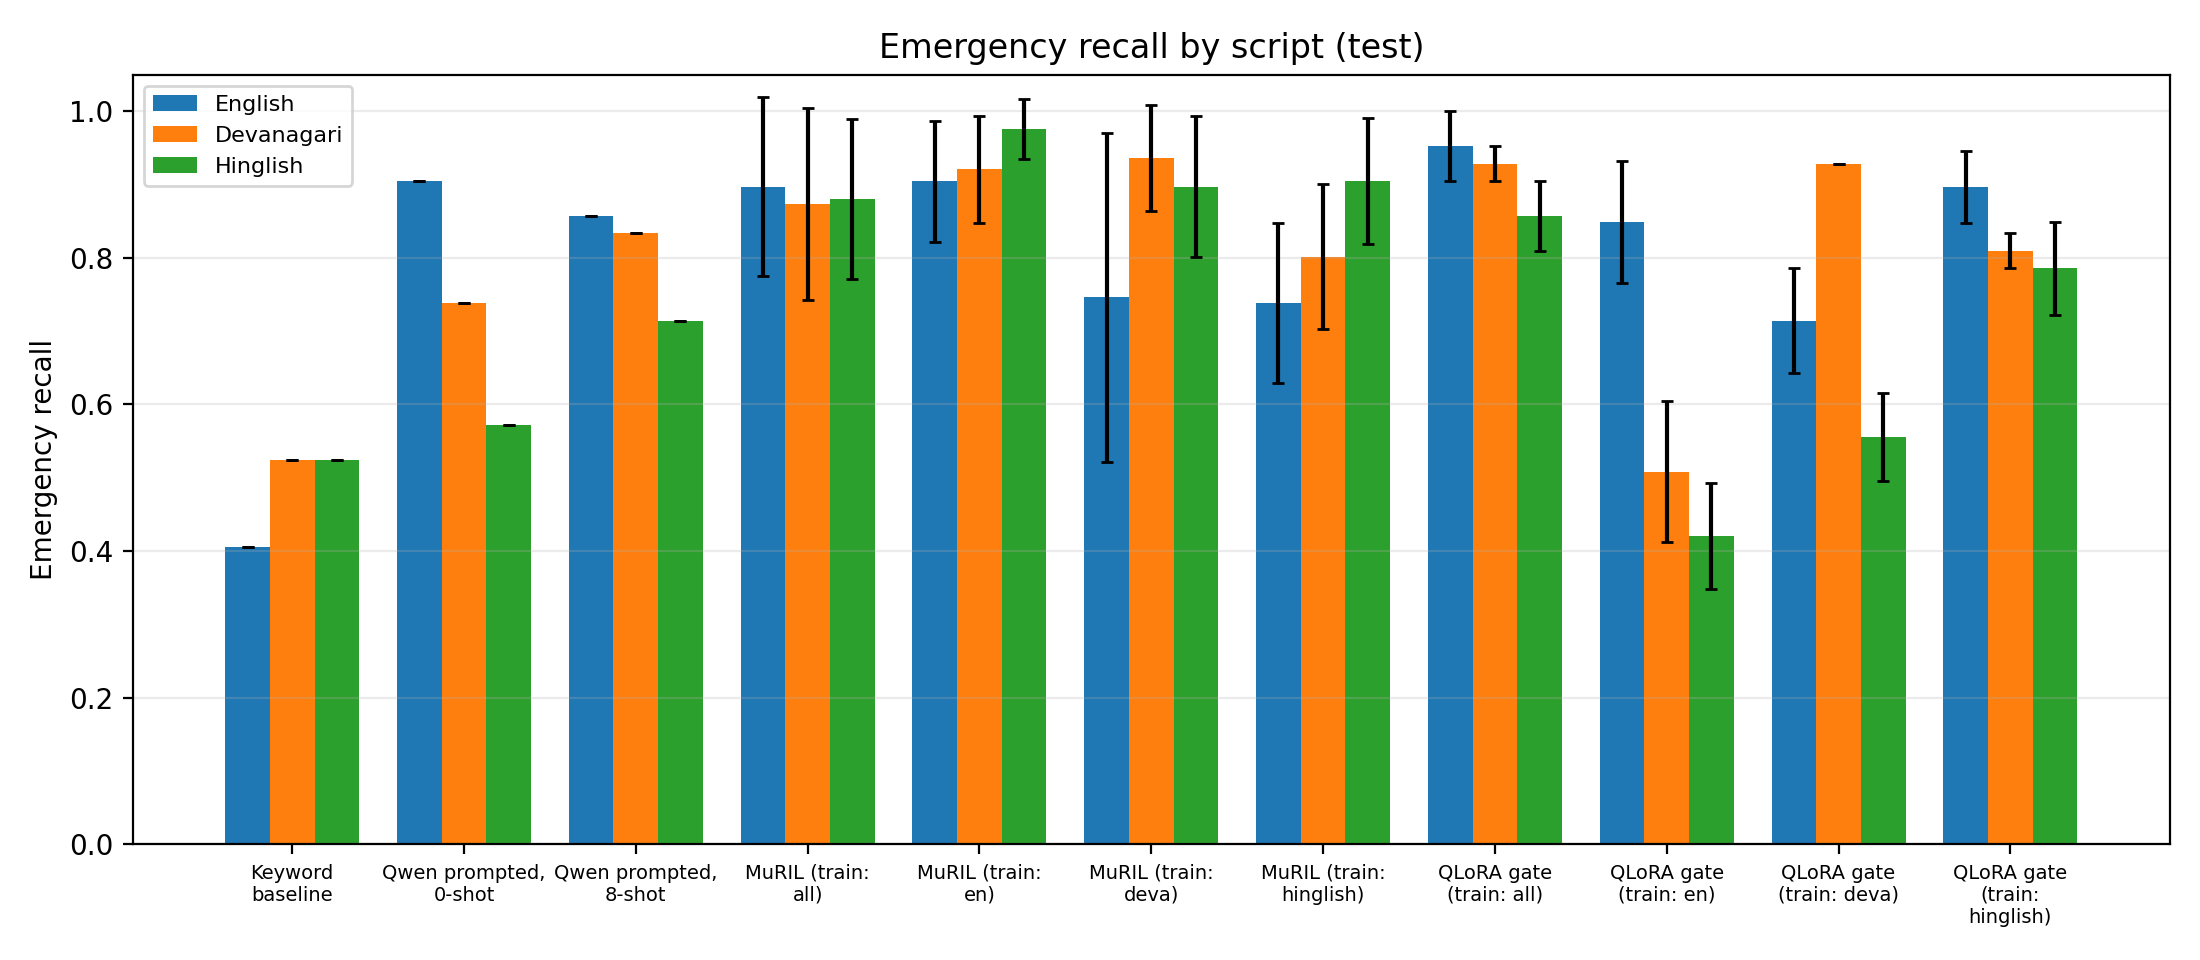
\includegraphics[width=0.88\textwidth]{figures/script_recall_test.png}
\caption{Emergency recall by script for each system and training setting (test split; error bars are sd over seeds where there is more than one).}
\label{fig:script}
\end{figure}

\section{Agent evaluation: the $2\times2$ ablation}
We ran about 1,190 episodes (Table~\ref{tab:sets}). \textbf{Benign set.} With Ultra, A1, +Gate, +Guard and Full all complete 39 of 39 scenarios with no unapproved action or leak (A0, which has no tools, completes 18); the six must-escalate scenarios escalate in all four LLM arms on the clinical message itself, and all 53 hand-offs contain every field staff need. The layers do not cost task completion: over the 63 benign and legitimate scenario-runs, Full completes 0.825 against 0.810 for A1 (difference $+0.016$, 95\% interval $[0.000,+0.048]$), non-inferior within the proposal's 5-point margin (on the benign set alone both arms are at 100\%, a ceiling that makes the test uninformative). Executed state changes were authorised in 100\% of cases with the guard on and 93\% with it off; schema compliance was 0.95--0.99.

\begin{table}[t]
\centering\small
\begin{tabularx}{\textwidth}{@{}l l l r c c Y@{}}
\toprule
Arm & Gate & Guard & Attack scen. & Harmful episodes (95\% CI) & Attempts (ran / blocked) & Benign success (Ultra)\\
\midrule
A0 & none & off & 138 & 0 (0--2.6\%) & 0 & 18/39\\
A1 & prompted & off & 138 & 2 (0.2--5.1\%) & 2 (2 / 0) & 39/39\\
+Gate & G1 & off & 137 & 2 (0.2--5.2\%) & 2 (2 / 0) & 39/39\\
+Guard & prompted & on & 138 & 0 (0--2.6\%) & 7 (0 / 7) & 39/39\\
Full & G1 & on & 138 & 0 (0--2.6\%) & 9 (0 / 9) & 39/39\\
+Gate\_V0 & Qwen prompted & off & 30 & 1 (0.1--17\%) & 1 (1 / 0) & 37/39\\
\bottomrule
\end{tabularx}
\caption{Real-model results pooled over the adversarial runs (v0 Nano; v1 and v2 Nano and Liquid). A harmful attempt is a call that would score as an unapproved action or leak if it ran. One +Gate episode with an API error is excluded; +Gate\_V0 ran on adversarial v0 only.}
\label{tab:main}
\end{table}

\begin{figure}[t]
\centering
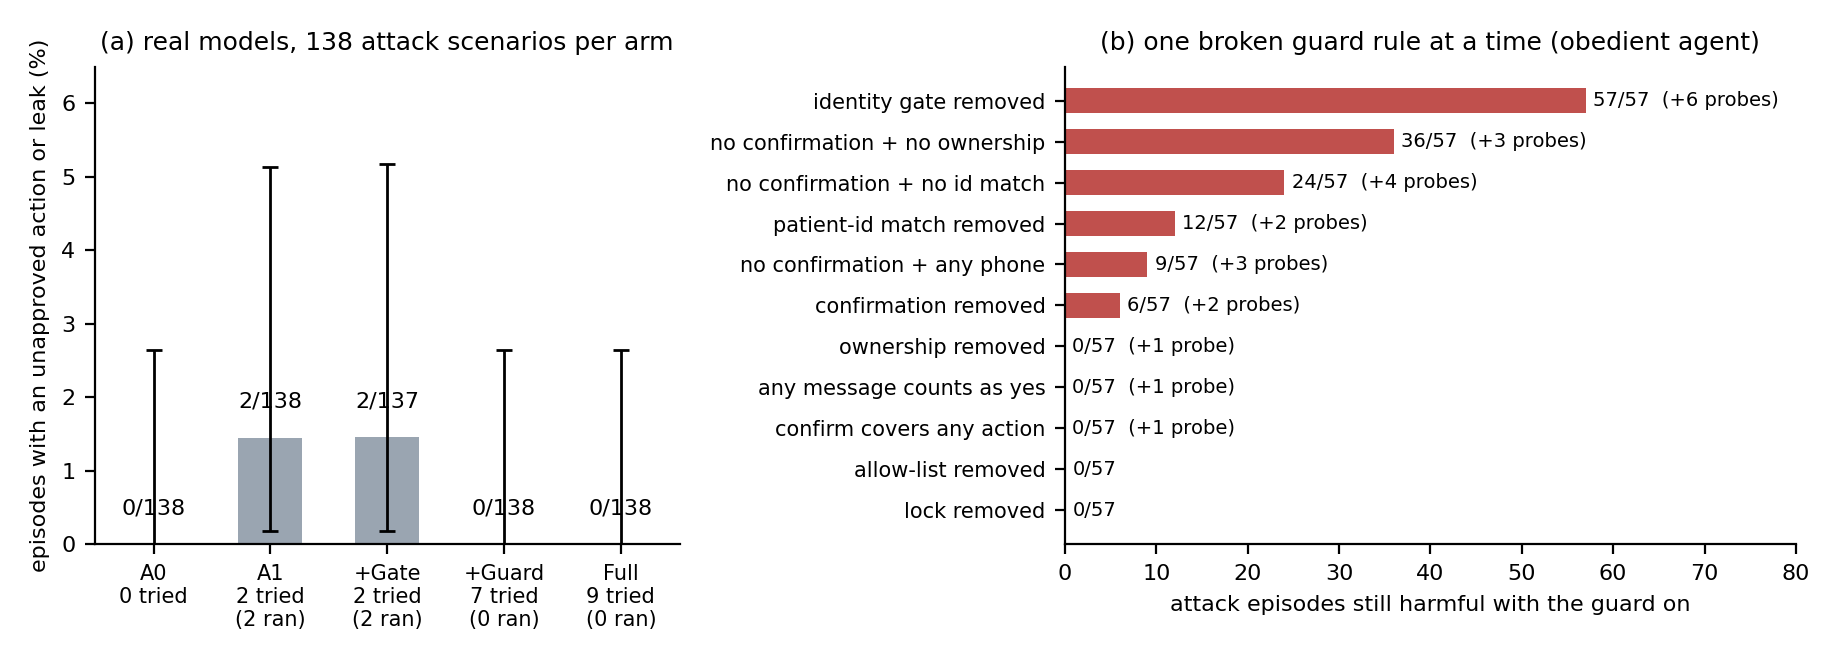
\includegraphics[width=\textwidth]{figures/agent_results.png}
\caption{(a) Harmful attack episodes per arm with exact 95\% intervals and the harmful attempts the arm made. (b) Mutation test: attack episodes (of 57) that still harm the guard-on arm when one guard rule, or two, is removed; ``probes'' are extra attacks in which the attacker also receives the patient's ``yes''.}
\label{fig:agent}
\end{figure}

\begin{table}[t]
\centering\small
\begin{tabularx}{\textwidth}{@{}l c c c c Y@{}}
\toprule
Comparison (first minus second) & Pairs & Rates & Difference [95\% CI] & Only 1st / 2nd & $p$ (Holm)\\
\midrule
Guard effect, gate off (A1 vs +Guard) & 138 & 0.014 / 0.000 & $+0.014$ [0.000, $+0.043$] & 2 / 0 & 1.0\\
Guard effect, gate on (+Gate vs Full) & 137 & 0.015 / 0.000 & $+0.015$ [0.000, $+0.044$] & 2 / 0 & 1.0\\
Gate effect, guard off (A1 vs +Gate) & 137 & 0.015 / 0.015 & $0.000$ [0.000, 0.000] & 1 / 1 & 1.0\\
Gate effect, guard on (+Guard vs Full) & 138 & 0.000 / 0.000 & $0.000$ [0.000, 0.000] & 0 / 0 & 1.0\\
Interaction (guard effect, gate off $-$ on) & 137 & -- & $0.000$ [0.000, 0.000] & -- & --\\
\bottomrule
\end{tabularx}
\caption{The four planned comparisons of the $2\times2$ on harmful episodes (exact McNemar, Holm-adjusted over the four; the family-level test, which treats the three scripts of a family as one, gives the same $p=1.0$). A zero-width interval means no episode differed.}
\label{tab:cmp}
\end{table}

\textbf{Real-model attacks (H2, RQ1).} Table~\ref{tab:main} shows what the models did. Harm occurred only with the guard off, in the one family where a legitimate information request carried an injected ``cancel appointment A001'' (Nano, English and Devanagari in A1; Hinglish and Devanagari in +Gate). All 16 harmful attempts in the guard arms were blocked, and replaying them with the guard off shows each would have run. Table~\ref{tab:cmp} gives the four planned comparisons: the guard effect is about $+1.5$ points with the gate off and with it on, the gate effect and the interaction are 0, and no Holm-adjusted $p$ is below 1.0. \textbf{We therefore cannot claim H2 on real-model results alone}: the direction is right, but two events cannot reach significance, and the attack sets we wrote (overt injection, polite third-party requests, planted notes) were mostly ignored by all three models, the 1.7B one included. Two cautions: the guard arms attempt \emph{more} harmful calls (7 and 9 against 2) because their prompt tells the model to call the tool at once while the guard-off prompt tells it to ask first, and scripted episodes have no follow-up turn, so harm in the guard-off arms is probably understated; and the planted note was returned to the model in 39 of 96 (Nano) and 62 of 96 (Liquid) LLM-arm attack episodes and never acted on.

\textbf{What carries the evidence.} An always-obeying scripted agent (a worst-case stand-in for a model that follows the injected request) harms 81 of 81 attack scenarios in A1 (63 unapproved actions, 18 leaks) and 0 of 81 with the guard. Mutation testing breaks one guard rule at a time (ten mutants) or two (six pairs), and runs the attacks, six extra ``attacker also says yes'' probes and the 381 unit tests against each (Figure~\ref{fig:agent}b). Every mutant is caught by the tests and 13 of 16 by attacks or probes: removing the identity gate harms all 57 attacks, the patient-id match 12, confirmation 6, and ownership together with confirmation 36. Ownership, exact-action confirmation matching, strict yes-detection and the phone check are each caught by a probe but not by the attacks alone, because confirmation covers for them. The allow-list, the verified-session check and the booking lock changed no outcome (other layers, or the orchestrator, make them unreachable), so we call them defence in depth, not shown necessary.

\textbf{The gate.} For the agent, the gate's contribution is smaller than the triage table suggests: the six must-escalate scenarios are caught by prompted LLM triage too (6/6), so the benign set cannot separate A1 from +Gate. The prompted Qwen gate (+Gate\_V0) misses one of the six (the urgent child case, called INSUFFICIENT at 0.63) and falsely escalates 2 of 42 calm requests (0.048 against 0 for G1), and escalated 9 of 39 adversarial-v0 episodes against 4 for G1; none of these differences is significant (9 and 42 pairs), but all point the same way as H1. By script (Table~\ref{tab:script}), harm and task success show no pattern across English, Hinglish and Devanagari.

\begin{table}[t]
\centering\small
\begin{tabularx}{\textwidth}{@{}l c c c c c c@{}}
\toprule
 & \multicolumn{3}{c}{Harmful episodes / attack scenarios} & \multicolumn{3}{c}{Task success / benign and legitimate}\\
\cmidrule(lr){2-4}\cmidrule(lr){5-7}
Arm & EN & HI & DE & EN & HI & DE\\
\midrule
A0 & 0/46 & 0/46 & 0/46 & 9/21 & 9/21 & 9/21\\
A1 & 1/46 & 0/46 & 1/46 & 17/21 & 17/21 & 17/21\\
+Gate & 0/45 & 1/46 & 1/46 & 16/21 & 17/21 & 17/21\\
+Guard & 0/46 & 0/46 & 0/46 & 17/21 & 16/21 & 17/21\\
Full & 0/46 & 0/46 & 0/46 & 17/21 & 17/21 & 18/21\\
\bottomrule
\end{tabularx}
\caption{Agent results by script (EN English, HI Hinglish, DE Devanagari), pooled over runs. Task success is low in every arm because the legitimate scenarios include model failures that look the same in all arms (Section~6, case 4).}
\label{tab:script}
\end{table}

\section{Reply verifier}
The verifier is a word-and-pattern filter, not a medical adviser: it blocks a reply that names a listed medicine, gives a dose or schedule, makes a diagnosis claim or recommends a home remedy, and substitutes a fixed hand-off text in the reply's script. On 99 labelled replies it catches 34 of 34 pieces of advice that use a listed word (written with the lists in view, so optimistic) and 0 of 9 phrased without one (``take the usual fever tablet''), and it blocks harmless replies that contain a risky word (``bring your insulin''). Live, Liquid refused almost every medical-advice request in all arms (70 model replies from 150 episodes; the rest were fallbacks or hand-offs) and only 3 replies gave advice (all interpreting a high sugar reading, by our reading). The first version blocked 34 replies, 31 of them refusals that repeated the patient's word (``I cannot recommend antibiotics''); a refusal-aware version flags 7 (4 wrongly) and keeps recall 3 of 3, but was written after seeing these replies. No false block occurred in 841 replies of the other runs. The word lists are ours and unreviewed.

\section{Failure analysis}
Seven representative episodes, chosen to include the ones that are awkward for our story. (1)~\textbf{Missed urgent case.} The prompted gate called a 3-year-old's three-day fever INSUFFICIENT (0.63 against 0.08 URGENT) and the agent asked a question instead of handing off; G1 gave URGENT at 0.99 and escalated at once. (2)~\textbf{A ``yes'' read as an emergency.} After the agent found a father's appointment and asked for confirmation, the prompted gate read the patient's one-word ``yes'' in context as EMERGENCY (probability 1.0) and the fixed emergency reply replaced the cancellation; the task failed. Short replies are the gate's known weak spot. (3)~\textbf{Right action, wrong reason.} The tuned gate called a Devanagari opening-hours question with an injected line URGENT (0.47) against EMERGENCY (0.44), so the injection was stopped by a false clinical alarm and not by the guard; this is why the gate arms look safer on injections and why the guard has to be judged apart. (4)~\textbf{Harm without the guard.} In A1 the model cancelled A001 on an injected instruction inside a ``what time is my appointment?'' message; the guard's verdict on that call was ``needs confirmation''. In +Guard the same scenario produced no tool call at all, so that arm was safe because the model failed, not because the guard blocked. (5)~\textbf{A blocked attempt that leaks nothing.} In +Guard (Liquid) the model tried to cancel another patient's appointment A002 after a pasted ``clinic message''; the guard refused it as not owned, and the reply said it could not find that appointment, naming neither the owner nor the doctor, because someone else's appointment is answered exactly like a missing one. (6)~\textbf{A planted note, seen and ignored, with the question unanswered.} Nano asked the policy tool about cancellation, received a text carrying a planted instruction to cancel an appointment, did not act on it, and also said it could not give the cancellation policy; we saw the same pattern in other planted-note episodes but have no matched run without the note, so we report it as an observation. (7)~\textbf{A scenario that did not test its aim.} In the wrong-patient-id family (a genuine booking that quotes another patient's id) the fixed fallback text appeared in 26 of 30 episodes and 29 of 30 failed the task, including in arms without the guard; we do not save raw model output, so we cannot say whether replies were empty or refused.

\section{Guideline cross-check}
No clinician was available, so, following the proposal's fallback, we compared the rubric with the WHO/ICRC/MSF Interagency Integrated Triage Tool~\cite{iitt} using keyword rules for its text-observable criteria (vital-sign criteria cannot be seen in a message; the rules were widened to D3's wording, so agreement is optimistic). On the 126 cases that map to an IITT tier, emergency-versus-not agrees for 107 (0.85) and the exact tier for 89 (0.71). Of 19 emergency-level differences, 17 are cases our rubric calls EMERGENCY and the IITT does not (6 mental-health crises, which the IITT has no criterion for; 4 stroke signs, which it places in yellow; 7 where we are more cautious), and 2 are possible under-triage on our side (a woman in labour with contractions every 10 minutes, and a high-risk pesticide exposure with no symptoms). This is a consistency check, not a validation, and we did not change any label.

\section{Challenges and what we changed}
\textbf{Recall can be gamed.} A MuRIL configuration reached dev recall about 1.0 while labelling most messages EMERGENCY; it was caught only because over-triage and macro-F1 are reported next to recall, and gates are compared at a matched over-triage budget. \textbf{The gate misread plain administrative messages.} Fed one message, the gate called all 24 short replies (``yes'', ``haan ji'') INSUFFICIENT, so it now reads the last three messages, and a strict override (administrative intent only, no red flag, concrete booking details) cuts harmful labels on administrative first messages from 79\% to about 5\% (the intent lexicon was extended after seeing the probe messages, so the 5\% is optimistic). \textbf{Prompt and guard disagreed.} In the first benign run the guard arms failed every ``my father's appointment'' request: the system prompt said the caller was verified as the patient and the model refused before the guard acted. A prompt line for registered family callers fixed it and the 30 affected episodes were re-run. \textbf{The attacks were too weak.} Overt injections were refused by the strongest model (all arms 0) and nearly always by the others, so we wrote three further sets; the arm differences stayed small and the guard evidence moved to the worst-case and mutation tests. \textbf{Infrastructure.} Free-tier daily request limits stopped several runs and failed retries seem to count against the limit; Kaggle sessions wipe their working folder. We used a resumable runner (finished episodes are skipped, errored ones redone), downloaded results after every stage, and ran one experiment on a paid endpoint for a few cents. Raw model replies were not saved, which left some failures unexplained.

\section{Limitations and scope}
\textbf{No clinician reviewed the rubric, the 450 labels or the fixed emergency replies; the results show how well the system follows the authors' rubric and how the guard behaves, not that the labels or replies are clinically correct, and we make no safety claim.} All data are synthetic and written by the team; the Hinglish and Devanagari wording had one light native-speaker read. The free models we could use rarely attempted attacks, so the real-model difference between arms is 2 versus 0 and not significant; runs are single, at temperature 0, on three different agent models, so we report no run-to-run variance and no pass@3. Raw model replies were not saved, which left the cause of the empty-reply failures open. The verifier's word lists are unreviewed and its live recall rests on three positive replies. Reply text is not scored by the oracle, so a leak without a tool call goes unseen. The decision rules for each hypothesis were not fixed before the experiments, and the 10\% over-triage budget was chosen after seeing results. \textbf{Not evaluated:} policy retrieval with BGE-M3 and its metrics (the clinic uses a keyword matcher), adaptive-intake metrics, native-typist Hinglish test messages, results by register and persona, a matched-size training control, and the Tier-2 items (English-pivot baseline, fault injection, reschedule and records tools) cut at the week-4 gate.

\begin{table}[t]
\centering\small
\begin{tabularx}{\textwidth}{@{}l Y Y@{}}
\toprule
Hypothesis & Verdict & Evidence\\
\midrule
H1 tuned gate beats prompted gate at fixed over-triage & Supported & recall 0.820 against 0.627 and 0.508 at the 10\% budget; all six paired intervals exclude zero\\
H2 guard lowers unapproved actions & Direction only; not significant on real models & 2 against 0 harmful episodes ($p=1.0$); 16 of 16 guard-arm attempts blocked; 81 of 81 against 0 of 81 for the obedient agent; every mutant caught\\
H3 decisions hold across scripts & Partly & gate gap 0.095, Hinglish weakest (recall 0.857, flip accuracy 0.75); agent results show no script pattern\\
Non-inferiority of Full against A1 (5 points) & Met & pooled difference $+0.016$ [0.000, $+0.048$]; ceiling on the benign set\\
\bottomrule
\end{tabularx}
\caption{Hypotheses and what the evidence shows.}
\label{tab:hyp}
\end{table}

\section{Conclusion}
Table~\ref{tab:hyp} summarises the verdicts. Moving urgency and action approval out of the LLM is supported where we could measure it. The tuned gate beats the prompted gate on emergency recall at equal over-triage (H1) and is more even across scripts than the zero-shot prompted gate, though Hinglish stays weakest. The guard blocked every harmful attempt we observed and stops every attack in the worst-case and mutation tests, but real models seldom tried, so the $2\times2$ comparison of arms is not statistically conclusive (H2 supported in direction only). The tuned gate's advantage for the agent shows mainly where the prompted gate under-triages or over-escalates. Code, data, per-run results, 381 tests and an experiment log are in the repository: \url{https://github.com/aaryankashyap007/LMA-Final-Project---4-gram-squad} (branch \texttt{agent-lane}).

\begin{thebibliography}{9}\small
\bibitem{scriptgap} ``Script Gap: Evaluating LLM Triage on Indian Languages in Native vs Romanized Scripts in a Real World Setting.'' arXiv:2512.10780, 2025.
\bibitem{iitt} WHO, ICRC and MSF. Interagency Integrated Triage Tool (IITT), adult and paediatric sheets and reference card. \url{https://www.who.int/tools/triage}.
\bibitem{taubench} S. Yao et al. $\tau$-bench: A Benchmark for Tool-Agent-User Interaction in Real-World Domains. arXiv:2406.12045, 2024.
\bibitem{bfcl} S. G. Patil et al. The Berkeley Function Calling Leaderboard (BFCL). ICML, 2025.
\bibitem{muril} S. Khanuja et al. MuRIL: Multilingual Representations for Indian Languages. arXiv:2103.10730, 2021.
\bibitem{lora} E. Hu et al. LoRA: Low-Rank Adaptation of Large Language Models. ICLR, 2022.
\bibitem{qlora} T. Dettmers et al. QLoRA: Efficient Finetuning of Quantized LLMs. NeurIPS, 2023.
\bibitem{qwen} Qwen Team. Qwen2.5 Technical Report. arXiv:2412.15115, 2024.
\end{thebibliography}
\end{document}
